\documentclass{article}
\usepackage[utf8]{inputenc}
\usepackage{listings}
\usepackage{CJKutf8}
\usepackage{amsmath}
\usepackage{graphicx}
\usepackage[subsection]{placeins}
\usepackage[export]{adjustbox}

           
\usepackage{tikz}
\usetikzlibrary{trees,automata, positioning, arrows}




\tikzstyle{lightedge}=[blue]
\tikzstyle{mainedge}=[red,very thick]
\tikzstyle{inputBit}=[rectangle,fill=red, text=white]
\tikzstyle{outputBit}=[rectangle,fill=blue, text=white]
\tikzstyle{pointer}=[orange,->,dashed]

\lstdefinestyle{mystyle}{
    backgroundcolor=\color{backcolour},   
    commentstyle=\color{codegreen},
    keywordstyle=\color{magenta},
    numberstyle=\tiny\color{codegray},
    stringstyle=\color{codepurple},
    basicstyle=\ttfamily\footnotesize,
    breakatwhitespace=false,         
    breaklines=true,                 
    captionpos=b,                    
    keepspaces=true,                 
    numbers=left,                    
    numbersep=5pt,                  
    showspaces=false,                
    showstringspaces=false,
    showtabs=false,                  
    tabsize=2
}

\lstset{style=mystyle}


\title{Lab6 Report}
\author{b09901142 EE3 呂睿超}
\date{December 2022}

\usepackage{xcolor}

\definecolor{codegreen}{rgb}{0,0.6,0}
\definecolor{codegray}{rgb}{0.5,0.5,0.5}
\definecolor{codepurple}{rgb}{0.58,0,0.82}
\definecolor{backcolour}{rgb}{0.8,0.9,0.8}


\begin{document}
\begin{CJK*}{UTF8}{bsmi}
\maketitle

\section{Symbol Mapper}  
\quad The following points are some techniques I used to implement the function
\begin{enumerate}
    \item From the $d_{min}$ formula, calculate $E_b$
    \item Select the bitstring segment
    \item Gray coding
        \begin{enumerate}
            \item Use recursion to handle the hamming distance property
            \item Use xor function to implement
             \item Source that I refer to: 
             
             \emph{https://www.matrixlab-examples.com/gray-code.html} 
             \item The implementation of gray coding is in \emph{Appendix 1} 
        \end{enumerate}
    \item Calculate $A_m$    
    \item Example of the implementation of PSK symbol mapping is in \emph{Appendix 2} 
\end{enumerate}




\section{Decision(Symbol Demapper)}
\subsection{(a)} 
\begin{enumerate}
    \item For generating bitstring that is drawn from Bernoulli distribution, simply use random seed and observe if $seed > 0.5$ .
    \item The symbol sequence after mapping (without noise) is in the first figure of \emph{Appendix 3}
    \item Using the following function can create simulate a noised symbol sequence
    \begin{lstlisting}[language = Matlab]
%% receive noise
function output = receiver(sim_sym_seq,var,M)
    le = size(sim_sym_seq,2)/log2(M);
    for i = 1:le
        nx = normrnd(0,var);
        ny = normrnd(0,var);
        noised_x(i) = sim_sym_seq{i}(1) + nx;
        noised_y(i) = sim_sym_seq{i}(2) + ny;
    end
    for i = 1:size(noised_x,2)
        output{1,i} = [noised_x(i),noised_y(i)];    
    end
end
    \end{lstlisting}
    \item normrnd is a function that can draw a random number from Gaussian distribution.
    \item calculating
    
    $d_{min} = 1  = 2\sqrt{\log_{2}{M}\sin^2{\frac{\pi}{M}}E_b}$ 
    
    $E_b = \frac{1}{4}$ 

    $\frac{E_b}{N_0} = 10dB$(for example)

    $\frac{E_b}{N_0}  = 10^{\frac{10}{10}} = 10$

    $N_0 = \frac{1}{40}$
    \item plug each $N_0$ to the variance and then we can generate the three figures in \emph{Appendix 3}
    
\end{enumerate}

\subsection{(b)}
\quad The following points are some techniques I used to implement the function
\begin{enumerate}
    \item I calculated the position of each constellation point.
    \item I generated a look up table of gray coded sequence for the last procedure of demapping.
    \item Using brute force to calculate the distance of the current processing symbol to each constellation point.
    \item Find the minimum of all distances and use the index to demap.
    \item The SER result of setting N0 = $\frac{1}{4}$ and mapping = 'PSK' is 0.0452(4.52\%) 
\end{enumerate}



\section{Error Probability and SNR}
\subsection{(a)(b)(c)}
\begin{enumerate}
    \item Since the implementation of (a) to (c) is similar, I'd write my viewpoints together.
    \item First, generate x data\_points which is $\frac{E_b}{N_0}$ and turn dB form to decimal form.
    \item Use for loop to iterate each experimenting scenario.
    \item The whole procedure is : generate\_binary\_seq $->$ symbol\_mapper $->$ receiver(simulate noised channel) $->$ symbol\_demapper $->$ calculate\_SER

    I wrote them all in functions respectively.
    \item Next, follow the hint, calculate the thereotical curve and plot all the curves and points on the figure.
    \item The figures are in \emph{Appendix 4}
\end{enumerate}

\subsection{(d)}
\begin{enumerate}
    \item Since the implementation of (a) to (c) is similar, I'd write my viewpoints together.
    \item First, generate x data\_points which is $\frac{E_b}{N_0}$ and turn dB form to decimal form.
    \item Use for loop to iterate each experimenting scenario.
    \item The whole procedure is : generate\_binary\_seq $->$ symbol\_mapper $->$ receiver(simulate noised channel) $->$ symbol\_demapper $->$ calculate\_SER

    I wrote them all in functions respectively.
    \item Next, follow the hint, calculate the thereotical curve and plot all the curves and points on the figure.
    \item The figures are in \emph{Appendix 4}
\end{enumerate}

\section{Convolutional codes + BPSK soft decoding}
\subsection{(a)}
\begin{enumerate}
    \item The whole procedure is : generate\_binary\_seq $->$ BPSK soft symbol\_mapper $->$ receiver(simulate noised channel) $->$ symbol\_demapper $->$ convolution\_decoder $->$ calculate\_BER
    \item The resulting figure is in \emph{Appendix 5}
    \item I believe that the figure is wrong because some part of the conv\_decoder in the implementation doesn't fit the scenario here.
\end{enumerate}

\subsection{(b)}

\section{Appendix}
\subsection{The implementation of gray coding}
\begin{lstlisting}[language = Matlab]
%% gray code function
function g = graycoding(b)
    g(1) = b(1);
    for i = 2 : length(b)
        x = xor(str2num(b(i-1)), str2num(b(i)));
        g(i) = num2str(x);
    end
end
\end{lstlisting}
\subsection{the implementation of PSK symbol mapping}
\begin{lstlisting}[language = Matlab]
    if(strcmp(name,'PSK'))
        sqrt_Ep = d/(2*sin(pi/M));
        l = log2(M);
        for i = 1:strlength(bin_seq)/l
            temp = bin_seq((i-1)*l+1:i*l);
            %disp(temp)
            gray_encoded_m = bin2dec(graycoding(temp));
            %disp(gray_encoded_m);
            Amx = cos((2*pi*(gray_encoded_m)+pi)/M);
            Amy = sin((2*pi*(gray_encoded_m)+pi)/M);
            
            sym_seq{i} = [Amx*sqrt_Ep,Amy*sqrt_Ep];
        end
    end
\end{lstlisting}
\pagebreak
\subsection{the figures of \emph{question 2a}}

\begin{figure}[!htb]
    \centering
    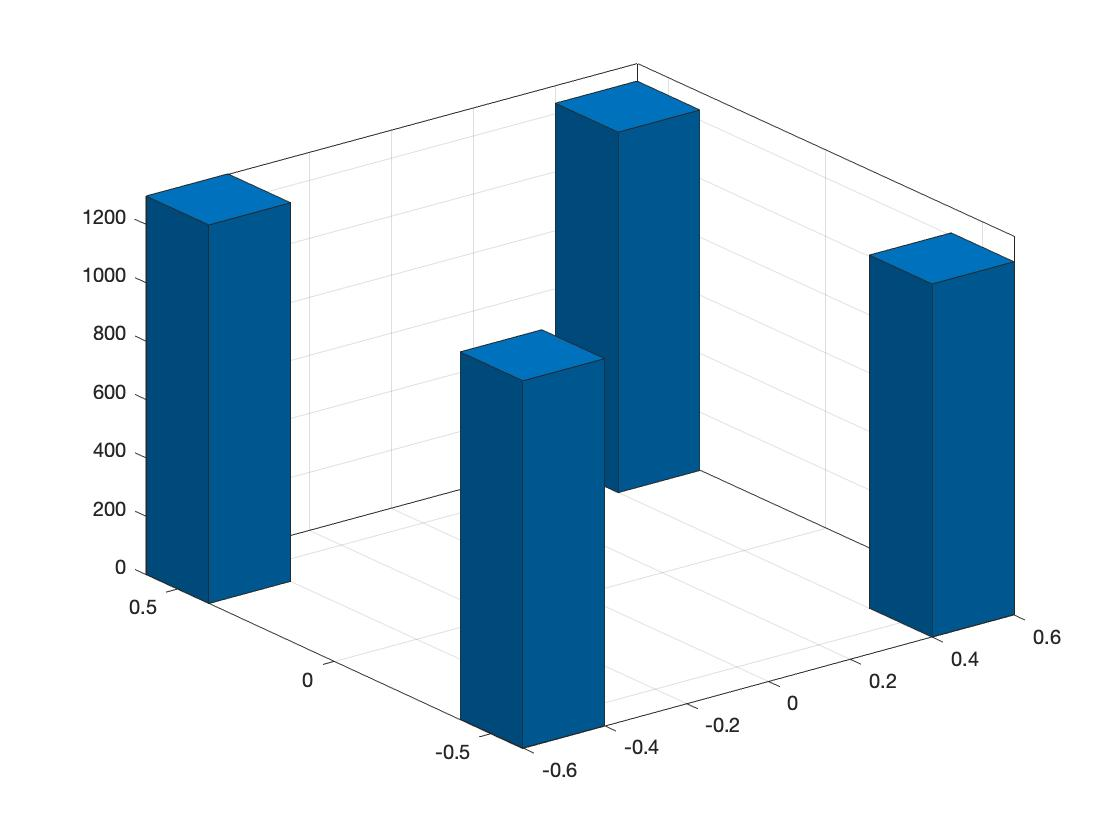
\includegraphics[width=0.7\textwidth]{2a_no.jpg}
    \caption{\label{fig:2a_no.jpg} No noise}
    \end{figure}
    \begin{figure}[!htb]
    \centering
    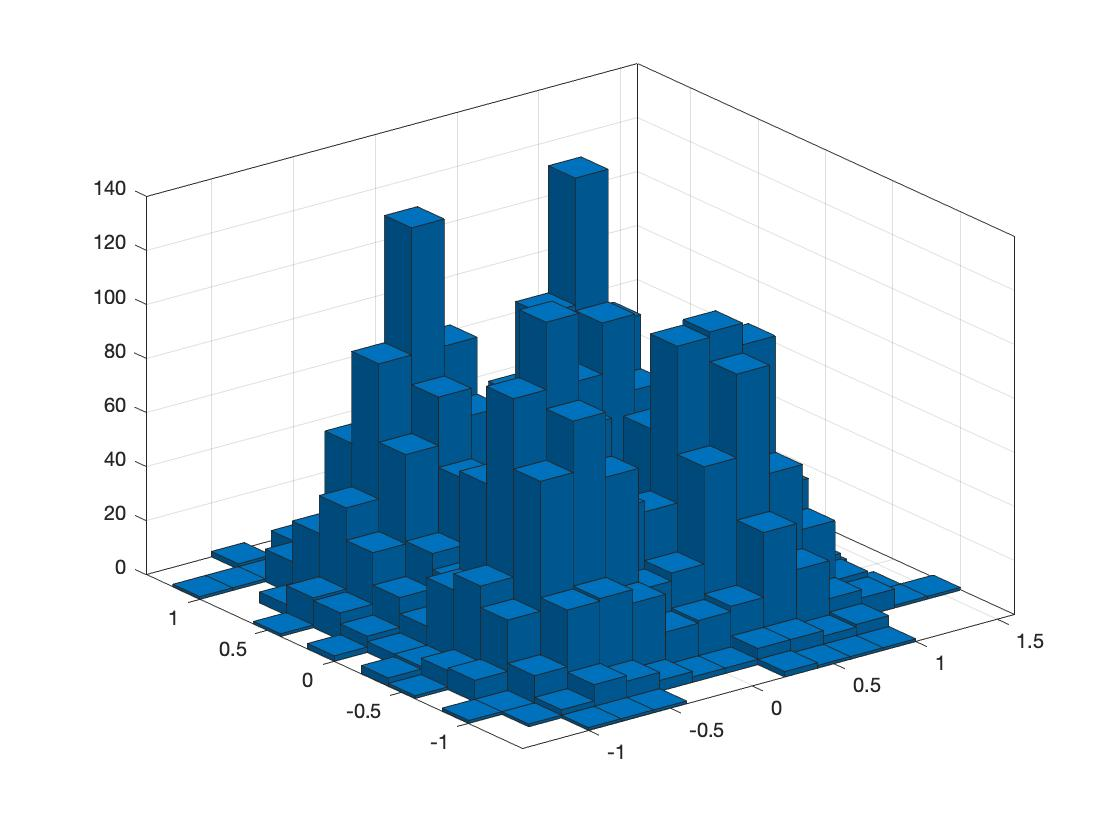
\includegraphics[width=0.8\textwidth]{2a_0.jpg}
    \caption{\label{fig:2a_0.jpg} Eb/N0 = 0 dB}
    \end{figure}
    \begin{figure}[!htb]
    \centering
    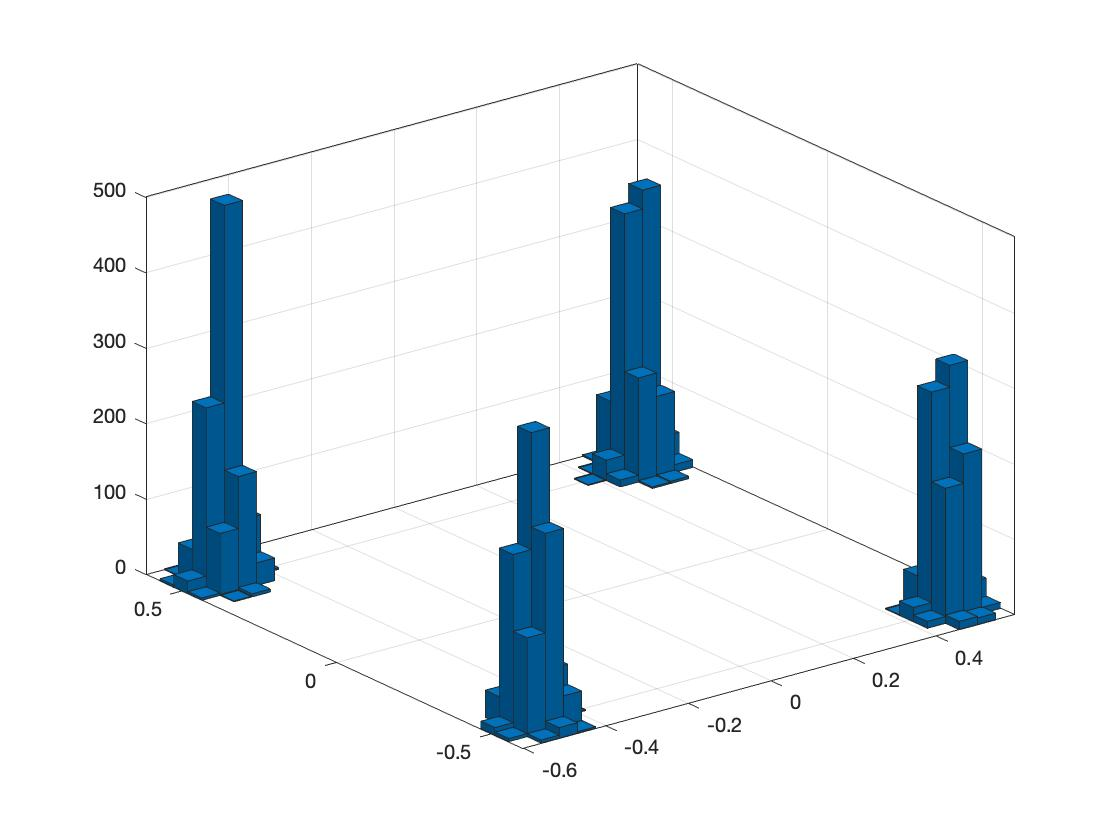
\includegraphics[width=0.9\textwidth]{2a_10.jpg}
    \caption{\label{fig:2a_10.jpg} Eb/N0 = 10 dB}
    \end{figure}
    \begin{figure}[!htb]
    \centering
    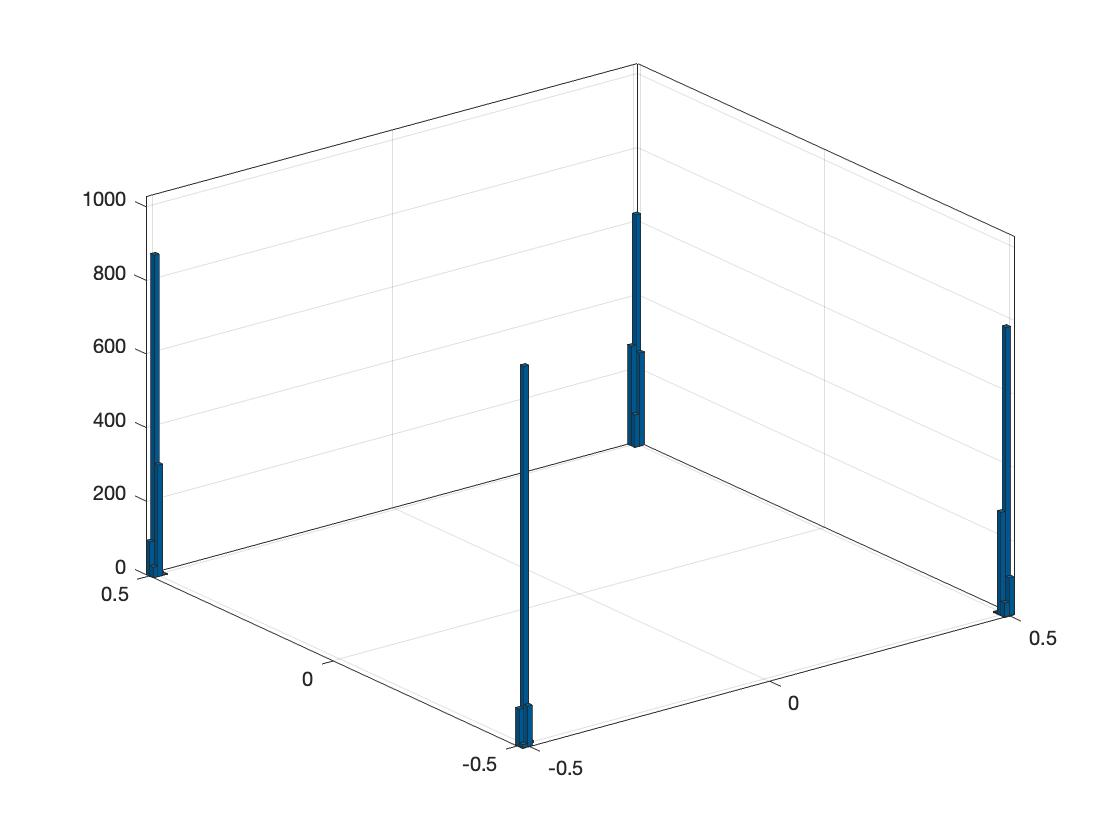
\includegraphics[width=0.9\textwidth]{2a_20.jpg}
    \caption{\label{fig:2a_20.jpg} Eb/N0 = 20 dB}
    \end{figure}

\pagebreak


\subsection{the figures of \emph{question 3}}
    \begin{figure}[!htb]
    \centering
    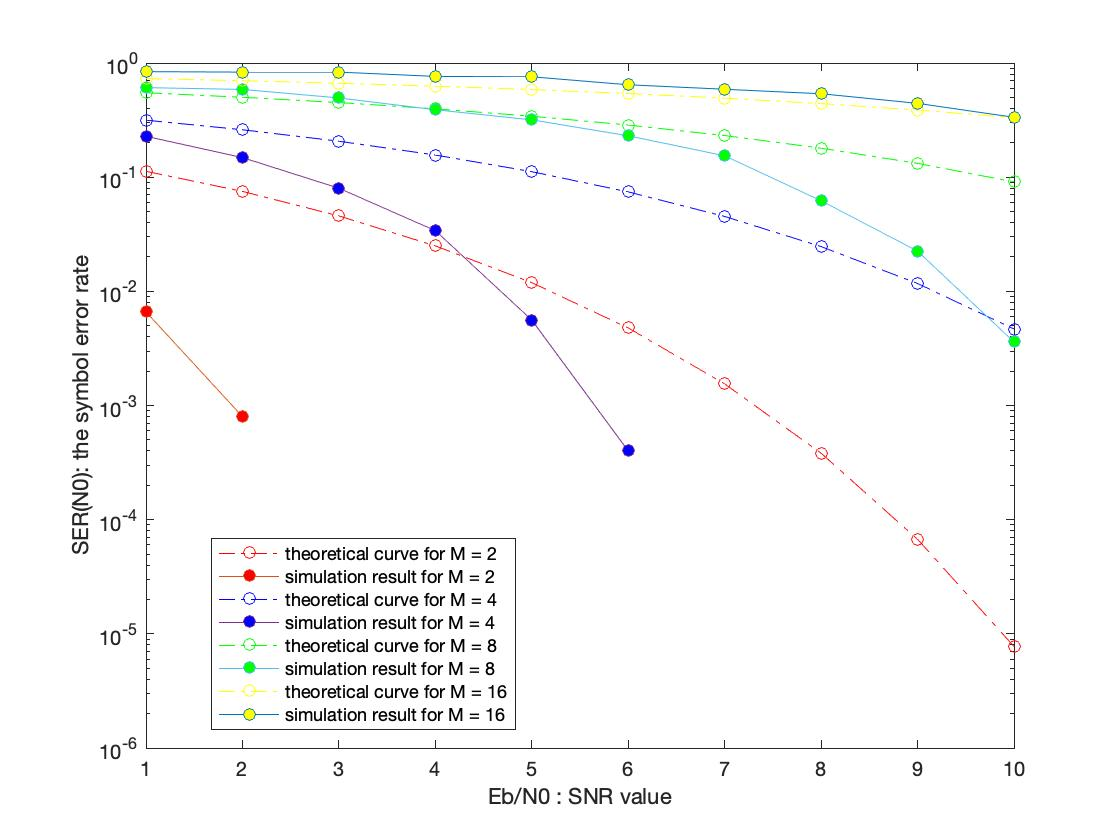
\includegraphics[width=0.8\textwidth]{PAM.jpg}
    \caption{\label{fig:PAM.jpg} PAM}
    \end{figure}
    \begin{figure}[!htb]
    \centering
    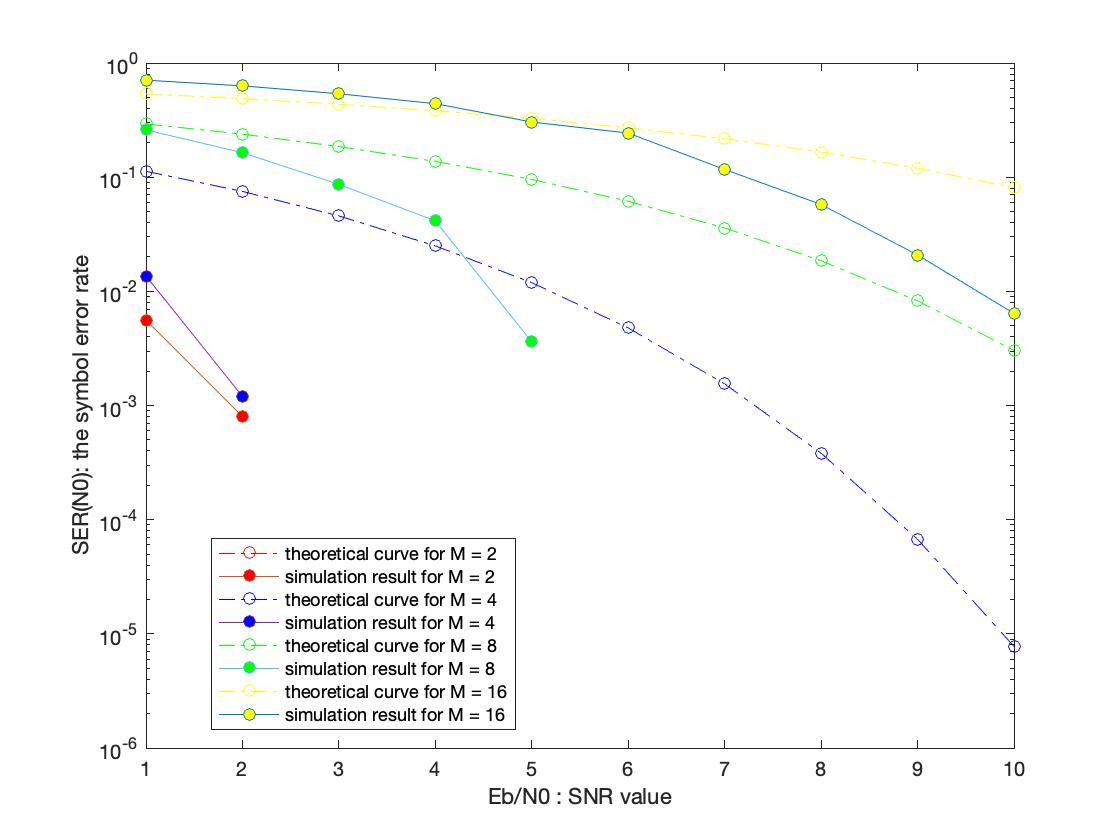
\includegraphics[width=0.8\textwidth]{PSK.jpg}
    \caption{\label{fig:PSK.jpg} PSK}
    \end{figure}
    \begin{figure}[!htb]
    \centering
    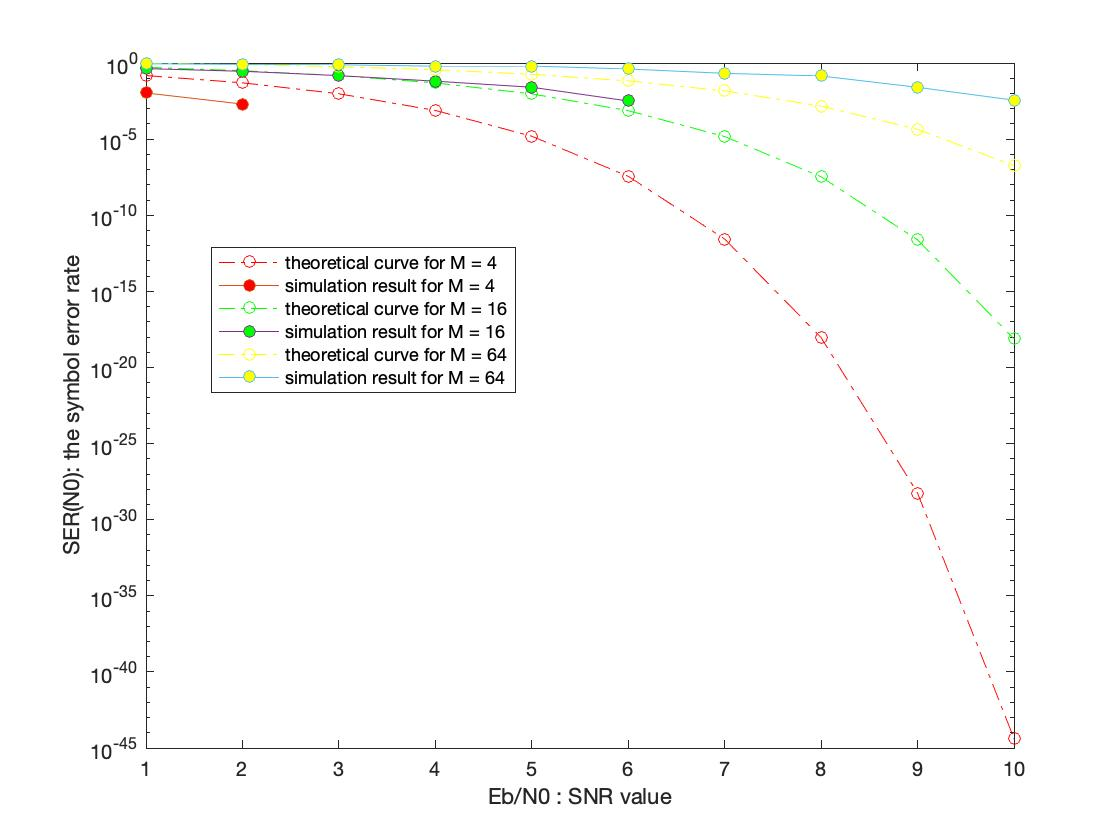
\includegraphics[width=0.8\textwidth]{QAM.jpg}
    \caption{\label{fig:QAM.jpg} QAM}
    \end{figure}
\pagebreak
\subsection{the figure of \emph{question 4}}
    \begin{figure}[!htb]
    \centering
    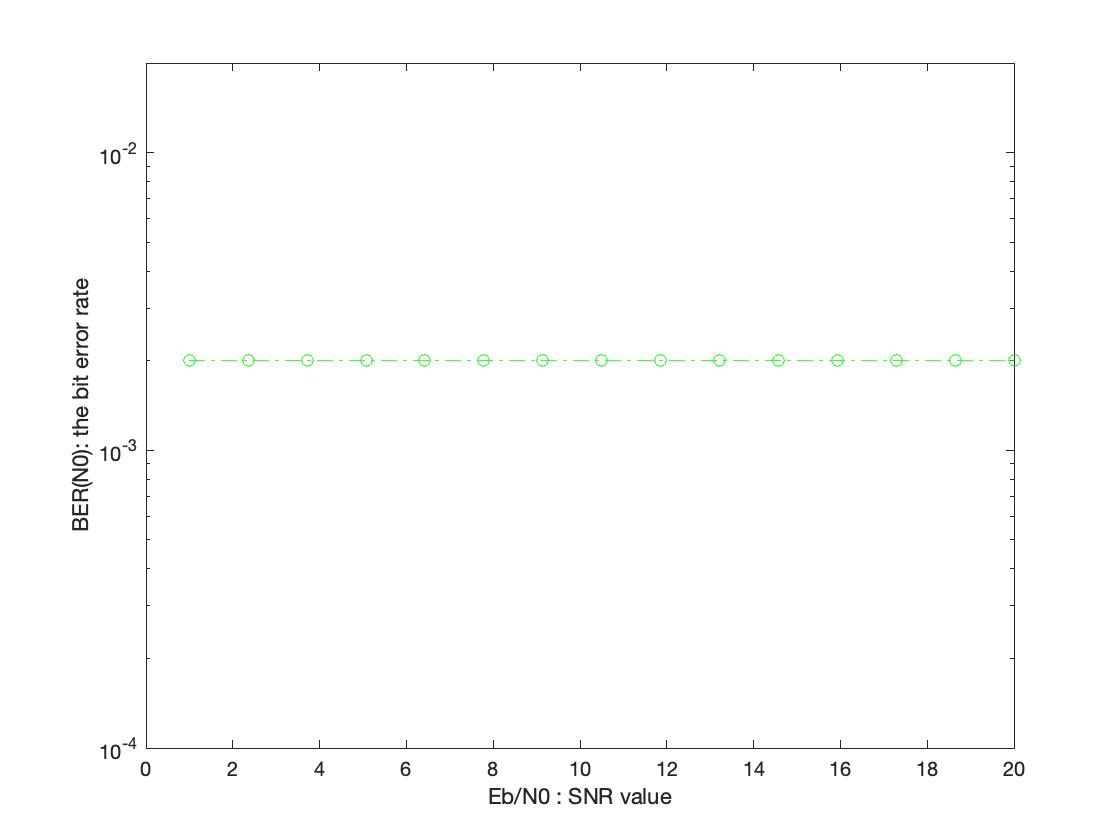
\includegraphics[width=0.8\textwidth]{4.jpg}
    \caption{\label{fig:4.jpg} the figure of \emph{question 4}}
    \end{figure}
\end{CJK*}
\end{document}
